\documentclass[class=book , crop=false, titlepage, twoside, multi={itemize, figure, verbatim}, float=false]{standalone}

\usepackage{import} % Required for importing other .tex docs.  (import uses everything bw Begin and End Doc)
\usepackage{float} % Required for specifying the exact location of a figure or table
\usepackage{graphicx} % Required for including images
\usepackage{wrapfig}
\usepackage[pdftex,breaklinks,colorlinks=true,linkcolor=black,citecolor=blue,urlcolor=red,linktocpage=false,pagebackref=true,filecolor=magenta]{hyperref}%http://www.tug.org/applications/hyperref/manual.html#x1-100003.6
\usepackage{cite}
\usepackage[toc,title,page]{appendix}
\usepackage{pdfpages} % enables loading a pdf into the doc
\usepackage{makeidx}
\usepackage{glossaries} % must be after hyperref
\usepackage{blindtext}
\usepackage{enumitem}
%\usepackage{caption}

%\setlist[description]{leftmargin=\parindent,labelindent=\parindent}

%\renewcommand*{\bibname}{References} % renames the bibliography

\newcommand{\HRule}{\rule{\linewidth}{0.5mm}} % Command to make the lines in the title page

\graphicspath{{img/}{GIS_ChampionSection/img/}{awardsChapter/GIS_ChampionSection/img/}{brandPart/awardsChapter/GIS_ChampionSection/img/}{img/}{pairedProgSection/img/}{methodChapter/pairedProgSection/img/}{methodPart/methodChapter/pairedProgSection/img/}{documentationSection/img/}{methodChapter/documentationSection/img/}{methodPart/methodChapter/documentationSection/img/}{docStorageOrgSection/img/}{methodChapter/docStorageOrgSection/img/}{methodPart/methodChapter/docStorageOrgSection/img/}{QGisSection/img/}{toolsChapter/QGisSection/img/}{servicePart/toolsChapter/QGisSection/img/}{ESRISection/img/}{toolChapter/ESRISection/img/}{servicePart/toolChapter/ESRISection/img/}{../../../../source/}{../../source/}{servicePart/applicationsChapter/treasurerSection/img/}}

%\setlength\parindent{0pt} % eliminates indents


\def\titlename{Map Services\\ \medskip\large Managing Map Services in ArcGIS}

\title{\HRule % Horizontal Line added
\\[.4cm] % space
\begin{figure}[H] % included image
\begin{center}	% centered horizontally

\includegraphics[scale=.45]{GIS_Logo_better.jpg}
\end{center}
\end{figure}
\Huge \bfseries \titlename \\ % Title text
\HRule \\[.4cm] % Horizontal Line added
\author{\Large Allegan County GIS \\\Large www.allegancounty.org/gis} % defines author
}  % inputs common title
\setcounter{tocdepth}{5}  % subparagraph and down
\begin{document}% document begins

\ifstandalone
%\frontmatter % turns off chapter numbering and uses roman numerals for page numbers
\maketitle % creates title page and blank page after title page
\tableofcontents % creates TOC and blank page
\clearpage
%\mainmatter % turns on chapter numbering, resets page numbering and uses arabic numerals for page numbers
\fi

\subsection{Managing Map Services}
\medskip
\subsubsection[Stopping the Server]{To stop ArcGIS Server}

\paragraph*{Launch ArcGIS Server Manager}
\begin{figure}[h!]
\centering
    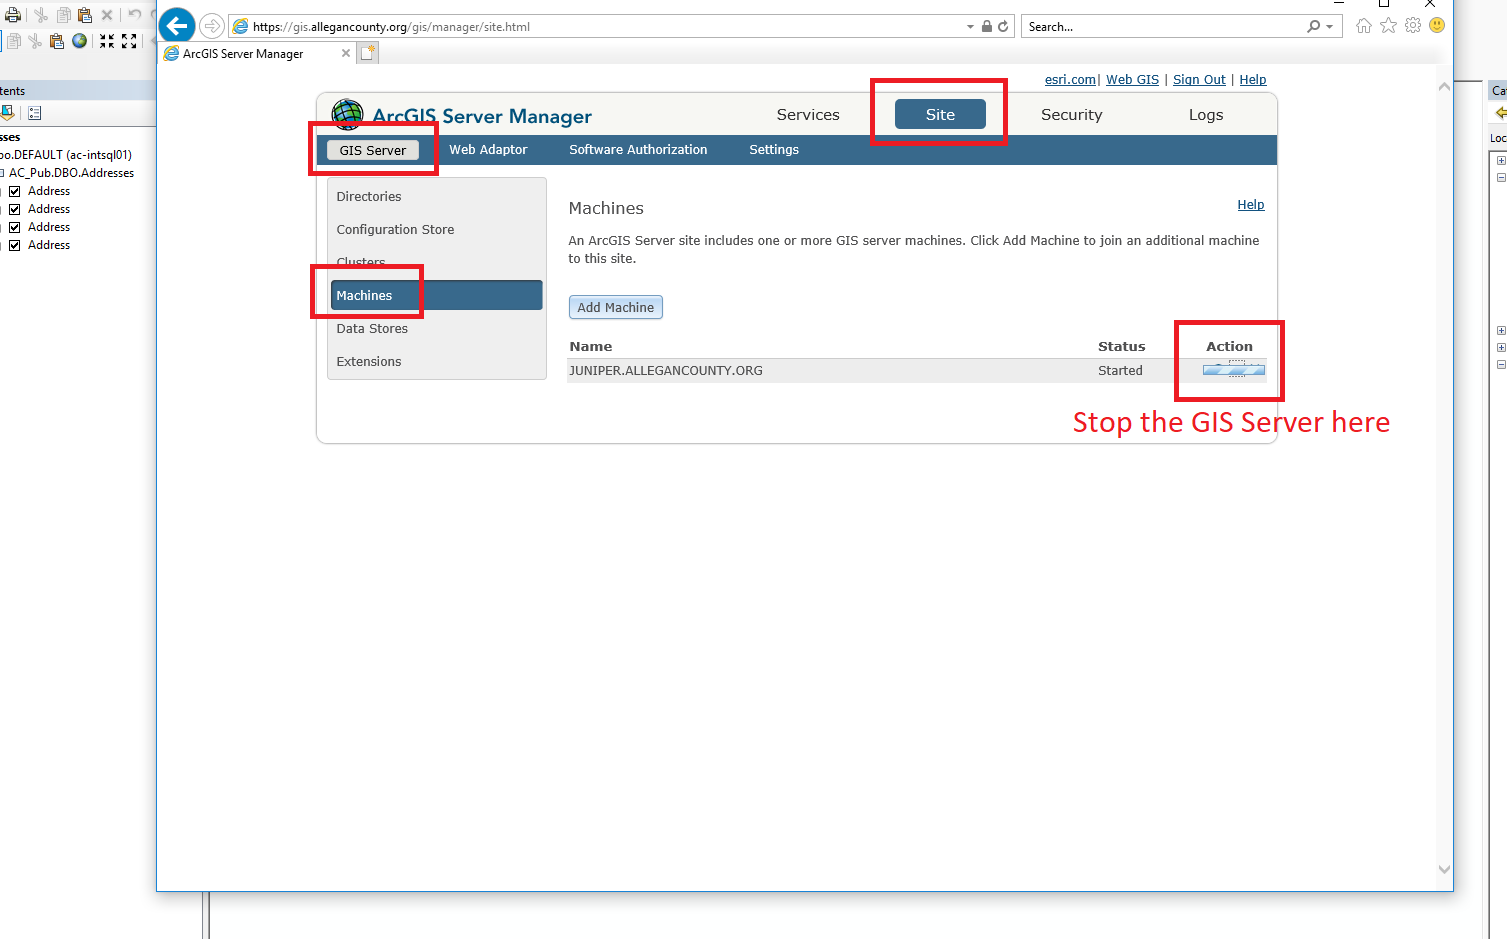
\includegraphics[width=.95\textwidth]{stopGisServer.png}
\caption{Stop the GIS Server}
\end{figure}

\subsubsection[Fixing Damaged Services]{\Large Fixing Damaged Services}

\paragraph[Remove Lock Files]{Removing Lock Files \texorpdfstring{\\}{}}
A blog about it
\href{https://community.esri.com/thread/103710}{https://community.esri.com/thread/103710}

\begin{verbatim}
on juniper
C:\arcgisserver\config-store\services\ParcelViewer2\
PV2Adresses.MapServer\startup\JUNIPER.ALLEGANCOUNTY.ORG

This method works.

Steps:

1)stop arcgis server services.

2)delete the lock files(*.glock and *.rlock )
    in arcgisserver\config-store.

3) restart arcgis server service.

4)stop the pending stopping service and then start it.
\end{verbatim}

\subsubsection[Running ArcGIS Server Account utility]{Running ArcGIS Server Account utility}

\paragraph[Error:]{Error: \texorpdfstring{\\}{}}

\textbf{Service is currently being configured by another administrative operation}


Remedy:
This tech support article applies:

\begin{verbatim}

https://support.esri.com/en/technical-article/000015549

\end{verbatim}

Our instuctions
Log into Juniper
windows R mstsc  juniper
Use personal network credentials


Launch the Configure ArcGIS Server account utility
ArcGISServerAccountUtility.PNG


Use these credentials
\begin{verbatim}
PW:  @lleganGIS2015
\end{verbatim}
in this:
AccountUtilityLogin.PNG


In the utility paste these paths:
gisDirectoryLocations.PNG
in this:


\begin{verbatim}

C:\arcgisserver\directories
C:\arcgisserver\config-store
C:\arcgisserver\logs
\end{verbatim}
like this:

gisDirectoryLocationsEntered.PNG


Do not export Config File
doNotExportConfigFile.PNG


press configure
configureAccount.png


Search For service Manger
searchForServiceManager.PNG


While the tool runs, open the service manager
windows  search services
openServicesManager.png


When the tool completes, press finish
then in services
select the ArcGIS Server service and restart the service.  (Randy had to do this)
arcGisServiceInServicesManager.png


mapservices would not stop so I try this:
\begin{verbatim}

https://support.esri.com/en/technical-article/000012685
\end{verbatim}

Check permission levels for the arcGIS account
ArcGisServerPermissions.PNG


If necessary, add the arcgis user to the permissions on the folders
ArcGisServerPermissionsAddUser.PNG






\end{document}
